\documentclass[]{article}
\usepackage{lmodern}
\usepackage{amssymb,amsmath}
\usepackage{ifxetex,ifluatex}
\usepackage{fixltx2e} % provides \textsubscript
\ifnum 0\ifxetex 1\fi\ifluatex 1\fi=0 % if pdftex
  \usepackage[T1]{fontenc}
  \usepackage[utf8]{inputenc}
\else % if luatex or xelatex
  \ifxetex
    \usepackage{mathspec}
  \else
    \usepackage{fontspec}
  \fi
  \defaultfontfeatures{Ligatures=TeX,Scale=MatchLowercase}
\fi
% use upquote if available, for straight quotes in verbatim environments
\IfFileExists{upquote.sty}{\usepackage{upquote}}{}
% use microtype if available
\IfFileExists{microtype.sty}{%
\usepackage{microtype}
\UseMicrotypeSet[protrusion]{basicmath} % disable protrusion for tt fonts
}{}
\usepackage{hyperref}
\PassOptionsToPackage{usenames,dvipsnames}{color} % color is loaded by hyperref
\hypersetup{unicode=true,
            pdftitle={Notes on Richard Stanley's Enumerative Combinatorics},
            pdfauthor={Tyler Neylon},
            colorlinks=true,
            linkcolor=black,
            citecolor=Blue,
            urlcolor=Blue,
            breaklinks=true}
\urlstyle{same}  % don't use monospace font for urls
\usepackage{longtable,booktabs}
\usepackage{graphicx,grffile}
\makeatletter
\def\maxwidth{\ifdim\Gin@nat@width>\linewidth\linewidth\else\Gin@nat@width\fi}
\def\maxheight{\ifdim\Gin@nat@height>\textheight\textheight\else\Gin@nat@height\fi}
\makeatother
% Scale images if necessary, so that they will not overflow the page
% margins by default, and it is still possible to overwrite the defaults
% using explicit options in \includegraphics[width, height, ...]{}
\setkeys{Gin}{width=\maxwidth,height=\maxheight,keepaspectratio}
\IfFileExists{parskip.sty}{%
\usepackage{parskip}
}{% else
\setlength{\parindent}{0pt}
\setlength{\parskip}{6pt plus 2pt minus 1pt}
}
\setlength{\emergencystretch}{3em}  % prevent overfull lines
\providecommand{\tightlist}{%
  \setlength{\itemsep}{0pt}\setlength{\parskip}{0pt}}
\setcounter{secnumdepth}{0}
% Redefines (sub)paragraphs to behave more like sections
\ifx\paragraph\undefined\else
\let\oldparagraph\paragraph
\renewcommand{\paragraph}[1]{\oldparagraph{#1}\mbox{}}
\fi
\ifx\subparagraph\undefined\else
\let\oldsubparagraph\subparagraph
\renewcommand{\subparagraph}[1]{\oldsubparagraph{#1}\mbox{}}
\fi
\usepackage{subfig}
\AtBeginDocument{%
\renewcommand*\figurename{Figure}
\renewcommand*\tablename{Table}
}
\AtBeginDocument{%
\renewcommand*\listfigurename{List of Figures}
\renewcommand*\listtablename{List of Tables}
}
\usepackage{float}
\floatstyle{ruled}
\makeatletter
\@ifundefined{c@chapter}{\newfloat{codelisting}{h}{lop}}{\newfloat{codelisting}{h}{lop}[chapter]}
\makeatother
\floatname{codelisting}{Listing}
\newcommand*\listoflistings{\listof{codelisting}{List of Listings}}

\title{Notes on Richard Stanley's Enumerative Combinatorics}
\author{Tyler Neylon}
\date{201.2016}

\begin{document}
\maketitle

These are somewhat informal notes I'm taking as I read through the book
\emph{Enumerative Combinatorics, Volume 1} by Richard P. Stanley
(Stanley 1997).

\section{Notes on chapter 1}\label{notes-on-chapter-1}

On page 19, we find the following proposition, which I quote directly:

\textbf{Proposition 1.3.4} Let \(x\) be an indeterminate, and fix
\(n\ge 0\). Then

\[\sum_{k=0}^n c(n,k) x^k = x(x + 1)(x + 2)\cdots (x + n - 1).\]

\begin{center}\rule{0.5\linewidth}{\linethickness}\end{center}

Three proofs are supplied for this proposition. I think the second proof
is not clearly written, so I'm going to dive into it a bit here.

\textbf{Clarified second proof of proposition 1.3.4}

Stanley defines \(F_n(x) := x(x + 1)(x + 2)\cdots (x + n - 1)\), which
I'll write as \(x^{\overline{n}}\) following Knuth's notation in
\emph{Concrete Mathematics} (Knuth, Patashnik, and Graham 1998). Given a
set \(I\) of intergers, I'll write \(\text{prod}(I)\) to denote the
product of all the elements of \(I\). In \(x^{\overline{n}}\), the
coefficient of \(x^{n-m}\), for \(m<n\), is

\[ \sum_{I \in \left\{{[n-1]\atop m}\right\}} \text{prod}(I). \]

In other words, it's the sum of all products of \(m-\)sets from
\([n-1]\). The claim of proposition 1.3.4 is that this is identical to
the value \(c(n,n-m)\).

We'll proceed by describing a procedure that results in an
\(n-\)permutation with exactly \(k=n-m\) cycles. Each different way of
carrying out this procedure results in a different permutation, and
every \(k-\)cycle permutation is produced by this procedure. In other
words, there are exactly \(c(n, k)\) ways to carry out this procedure.

This is the procedure: We'll begin with the string
\(s_0 = 1, 2, \ldots, n\) and move one item at a time around in the
string until we arrive at a target string. We can think of each string
as the standard order of a permutation's cycle notation; this is the
string-permutation correspondence mentioned in Stanley's proposition
1.3.1. The procedure has two parameters: a set \(I \subset [n-1]\) of
size \(|I| = m\), and a function \(g:I\to [n-1]\) satisfying
\(g(i) \le n - i\). Sort \(I\) so that \(I = i_1 > i_2 > \ldots > i_m\).
Then at the \(j^\text{th}\) step, start with string \(s_{j-1}\) and
alter it by moving \(i_j\) to the right by \(g(i_j)\) items, resulting
in string \(s_j\). At the end of step \(m\), we'll have the final string
\(s_m\).

\textbf{Example} Suppose \(n=4\), \(I=\{2,3\}\), \(g(2) = 2\), and
\(g(3) = 1\). Then the procedure would generate the following strings:

\[
\begin{array}{rcl}
s_0 & = & 1, 2, 3, 4 \\
s_1 & = & 1, 2, 4, 3 \\
s_2 & = & 1, 4, 3, 2 \\
\end{array}
\]

The first step moved 3 to the right by \(g(3)=1\) position; the second
step moved 2 to the right by \(g(2)=2\) positions. The final result
corresponds to the permutation \((1) (4\; 3\; 2)\), written in cycle
notation.

Our first job is to show that this process provides a bijection between
its parameters \((I, g)\) and the set of all \(k-\)cycles.

Suppose we have a \(k-\)cycle permutation \(\pi\) written in standard
cycle notation. Then each cycle has a \emph{leader}, which is the
largest element of that cycle. Denote these leaders as
\(t_1, t_2, \ldots, t_k\). Denote the remaining items, in decreasing
order, as \(i_1 > i_2 > \ldots > i_m\). Think of the first string
\(s_0\) as the identity permutation made up of \(n\) different 1-cycles.
The first step is to delete the 1-cycle containing \(i_1\) and to move
it into the cycle with its leader in \(\pi\). In the string, this
corresponds with moving \(i_1\) so that it's immediately after its
leader. This must be a nontrivial move to the right for \(i_1\). In
general, the \(j^\text{th}\) step involves removing the 1-cycle with
element \(i_j\), and placing that element in the appropriate spot with
the cycle owned by its leader in \(\pi\). This always corresponds to
moving \(i_j\) to the right in the standard order because \(i_j\) will
remain to the left of its leader until step \(j\), after which it will
be to the right of its leader. This shows that the above procedure can
produce any given \(k-\)cycle permutation.

In the other direction, any execution of the procedure that takes \(m\)
steps will result in a permutation with \(k=n-m\) cycles because each
step removes a single cycle from the permutation. To see this, note that
the set of elements to the right of \(i_j\) doesn't change before step
\(j\). Thus when \(i_j\) moves right, it must gain a new left-to-right
maximum element that becomes its leader. The cycle that gains \(i_j\) on
step \(j\) continues to have the same leader and to contain all its
previous elements as \(i_j\) must be the smallest element so far in that
cycle.

Note that our restriction on \(g\) is maintaining that each element
\(i_j\) must move to the right by at least one place, and may move at
most \(n-i_j\) positions to the right since the elements to the right of
it are exactly \(i_j + 1, i_j + 2, \ldots, n\).

This argument has shown that every pair \((I, g)\) maps to a \(k-\)cycle
permutation \(\pi\), and that this mapping is a bijection.

For given values of \(n\) and \(m\), how many pairs \((I, g)\) are
there?

We have two ways to count this set.

For a given set \(I\subset [n-1]\) with \(|I| = m\), let
\(A(I):=\{n - i \, | \, i \in I\}\). Then there are \(\text{prod}(A)\)
values of \(g\) that may be chosen that could pair with \(I\). Since
\(A: \left\{{[n-1]\atop m}\right\} \to \left\{{[n-1]\atop m}\right\}\)
is a bijection, the total number of \((I, g)\) pairs is

\[\sum_{I \in \left\{{[n-1]\atop m}\right\}} \text{prod}(A(I)) =
  \sum_{I \in \left\{{[n-1]\atop m}\right\}} \text{prod}(I).\]

By the bijection just explained, this value must also be the total
number of \(k-\)cycles, that is, exactly \(c(n, k)\); this is using that
\(k=n-m\), as above. We can summarize this by saying that

\[c(n, k) = \sum_{I \in \left\{{[n-1]\atop m}\right\}} \text{prod}(I).\]

The left expression is the coefficient of \(x^k\) on the left side of
proposition 1.3.4, while the right expression is the coefficient of
\(x^k\) on the proposition's right side. This completes the proof.

\textbf{Correspondence with the book's version of the proof} \(\quad\)
In the table below, I'm informally using the notation \(n-X\) on a set
\(X\) to denote \(\{n-x \,|\, x\in X\}\), or on a function \(X\) to
denote another function \(X'\) such that \(X'(x) = n - X(x)\).

\begin{longtable}[]{@{}lll@{}}
\toprule
My notation & \(\quad\) & Stanley's notation\tabularnewline
\midrule
\endhead
\(I = i_1, \ldots, i_m\) & & \(b_1, \ldots, b_m\)\tabularnewline
\(A(I) = n - I\) & & \(S\)\tabularnewline
\(g\) & & \(n - f\)\tabularnewline
\(t_1, \ldots, t_k\) & & \(T\)\tabularnewline
\bottomrule
\end{longtable}

\textbf{Notes on the third proof of proposition 1.3.4}

In the book, there is a small mistake: The book gives the condition
\(0 \le a_i \le x + n - i\), but it should really be
\(0 \le a_i \le x + n - i - 1\). That way, \(a_i\) can take on exactly
\(x + n - i\) possible values. Since \(i\) ranges from 1 to \(n\), there
are \(x^{\overline{n}}\) possible values for the sequence
\((a_1, \ldots, a_n)\).

This proof uses a slight variant of the same procedure I described
above. The procedure is augmented by treating my function \(g\) as a map
for all elements --- rather than just for a subset of them --- and by
adding a map from each \(z : g(z) = 0\) to some value in \([x]\). Since
each such \(z\) becomes the leader of a cycle, this corresponds with the
map the book presents as \(f:C(\pi) \to [x]\).

\begin{center}\rule{0.5\linewidth}{\linethickness}\end{center}

On page 20 is the following proposition, quoted directly:

\textbf{Proposition 1.3.7}

Let \(n, k\in\mathbb{P}\). The number of integer sequences
\((a_1, \ldots, a_n)\) such that \(0 \le a_i \le n-i\) and exactly \(k\)
values of \(a_i\) equal 0 is \(c(n, k)\).

\begin{center}\rule{0.5\linewidth}{\linethickness}\end{center}

The above proposition follows immediately by my discussion of the
procedure at hand. Specifically, that procedure generates \(k\) cycles
when the set \(\{z : g(z) > 0\}\) has size \(n - k\); that is, when the
set \(\{z : g(z) = 0\}\) has size \(k\). I phrased the last sentence
that way to make the connection with the variable \(m = n-k\) used in
the argument above --- specifically, the paragraph starting with ``In
the other direction,---.''

\begin{center}\rule{0.5\linewidth}{\linethickness}\end{center}

\textbf{Clarifications around proposition 1.3.12}

Shortly after that, the book presents a permutation in standard cycle
notation,

\[\pi = (a_1 a_2 \ldots a_{i_1}) \,
        (a_{i_1+1} a_{i_1+2} \ldots a_{i_2}) \, \cdots \,
        (a_{i_{k-1}+1} \ldots a_n).\]

It also works with \(\hat\pi\), the permutation achieved by dropping the
parentheses from the standard cycle notation of \(\pi\), and the
notation \(d(\hat\pi)\) for the number of descents --- places where
\(a_i > a_{i+1}\) --- in the permutation \(\hat\pi\).

I'm going to clarify the argument leading up to the equation

\begin{equation}n-d(\hat\pi) = \#\{i\in[n]:\pi(i)\ge i\}.\label{eq:num_desc_pi_hat}\end{equation}

The first claim to verify is that ``if \(\pi(a_i)\ne a_{i+1}\), then
\(a_i<a_{i+1}\).'' The precondition conceptually means that \(a_i\) is
is an end-of-cycle value. The consequence follows by the nature of
standard cycle notation --- cycle leader values are always greater than
their preceding value.

The second claim to verify is that

\begin{equation}a_i<a_{i+1}\text{ or }i=n \quad\Leftrightarrow\quad \pi(a_i)\ge a_i.\label{eq:pre_num_desc_iff}\end{equation}

I'll justify this using two cases. First, suppose \(a_i\) is an
end-of-cycle value. We saw in the last paragraph that this means the
left side is true; the right side is also true since \(\pi\) was written
in standard cycle notation, and \(\pi(a_i)\) is the leader of \(a_i\)'s
cycle. Next, suppose \(a_i\) is not an end-of-cycle value. Then \(i=n\)
is false, so we're looking at
\(a_i<a_{i+1}\,\Leftrightarrow\,\pi(a_i)\ge a_i,\) which is clearly true
since \(\pi(a_i) = a_{i+1}\) whenever \(a_i\) is not an end-of-cycle
value. This justifies (\ref{eq:pre_num_desc_iff}).

The jump from (\ref{eq:pre_num_desc_iff}) to (\ref{eq:num_desc_pi_hat})
is based on counting. Specifically, rewrite (\ref{eq:pre_num_desc_iff})
as

\[\#\{i:a_i<a_{i+1}\text{ or }i=n\} = \#\{i:\pi(a_i)\ge a_i\}.\]

The left side is the number of \(i\) which are non-descents in
\(\hat\pi\), in other words \(n - d(\hat\pi)\). That is, we've arrived
at (\ref{eq:num_desc_pi_hat}).

Next is the claim that ``a permutation \(\pi=a_1a_2\cdots a_n\) has
\(k\) weak excedences if and only if the permutation
\(b_1b_2\cdots b_n\) defined by \(b_i = n+1-a_{n+1-i}\) has \(n-k\)
excedences.'' Given the permutation with word \(a_1a_2\cdots a_n\), I'll
use the term \emph{flipped} to refer to the permutation with
\(i^\text{th}\) value \(n+1-a_i\), and the term \emph{reversed} to refer
to the permutation with \(i^\text{th}\) value \(a_{n+1-i}\). So the
claim is pointing toward a kind of partitioning of \([n]\) based on weak
excedences in a permutation versus excedences in its flipped reversal.
Figure~\ref{fig:excedence} gives a visual explanation of this
partitioning, which I hope adds some intuition to the claim.

\begin{figure}[htbp]
\centering
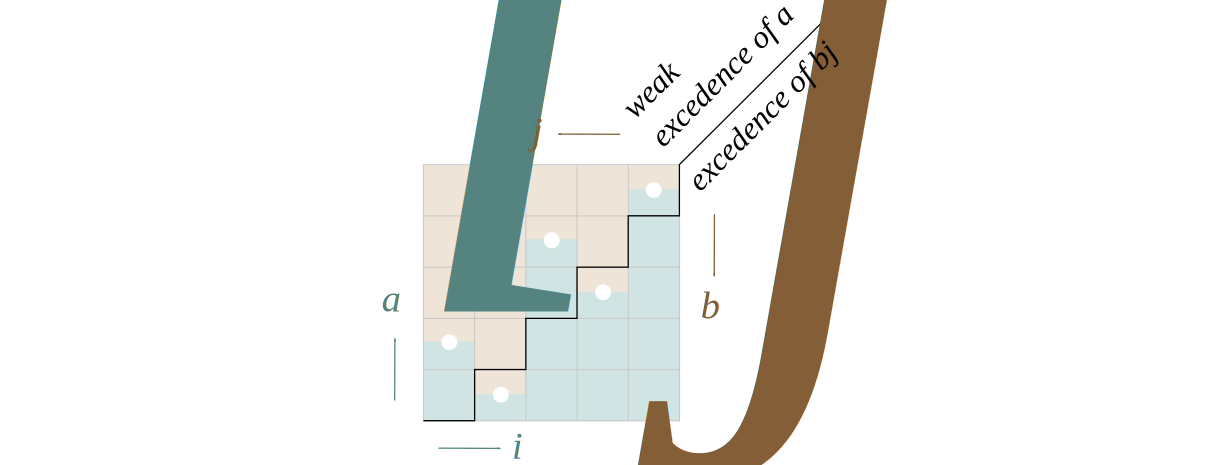
\includegraphics{images/pdfs/excedence.pdf}
\caption{\label{fig:excedence}This represents the permutation
\(\pi_a = 21435\) and its flipped reverse permutation \(\pi_b = 13254\).
Permutation values above the bold zig-zagging diagonal cut are weak
excedences of \(\pi_a\) while those below are excedences of
\(\pi_b\).}\label{fig:excedence}
\end{figure}

TODO rest of notes from my voice memo

\begin{center}\rule{0.5\linewidth}{\linethickness}\end{center}

\section*{References}\label{references}
\addcontentsline{toc}{section}{References}

\hypertarget{refs}{}
\hypertarget{ref-concrete}{}
Knuth, Donald E., Oren Patashnik, and Ronald L. Graham. 1998.
\emph{Concrete Mathematics: A Foundation for Computer Science}.
addison-wesley.

\hypertarget{ref-stanley}{}
Stanley, Richard P. 1997. \emph{Enumerative Combinatorics, Volume 1}.
Cambridge University Press.

\end{document}
